\section{Evaluation}
\label{sec:eval}

We perform some preliminary experiments to evaluate the effectiveness of AccWeb.

\subsection{Evaluation setup}

Our experiments are conducted using Chrome browser on a Macbook Pro laptop, running macOS Sierra, as the client. This client connects to a WiFi hotspot exported by a TP-LINK router. For simplicity, the client is both measuring agents for analyzing web resources and the user for browsing web pages. We load the full version of web pages using Google Chrome Version 55.0.2883.95 (64-bit) for Mac. We host Prefetcher and Analyzer in a small instance VM in Amazon EC2's US West Region. Predictor is a Chrome extension running on the client side. %Different experiments have small changes on the setup, which will be explained in the subsections below.


\subsection{Page Loading Time}

We evaluate the improvement in page loading times enabled by the full mode and the limit mode of AccWeb, compared with the loading times without AccWeb. We have two assumptions: first, we assume that our prediction is correct; second, we assume that before the user loads a web page, all static resources required to be prefetched are already loaded - when the browser starts to load web pages, the prefetched resources can be obtained from the cache. We select 50 websites from Alexa's top 150 websites in China, load 10 times for each web page, and record loading times of these websites in the full load mode, the limit mode, and non-prefetching mode. When testing non-prefetching mode, we disable Chrome's default prefetching service.



We plot the CDFs (across websites) of average loading times (Fig.~\ref{fig:average}) and CDFs of median loading times (Fig.~\ref{fig:median}) of the websites in the 3 different modes. As we can see from the plots, there are evident improvements in loading times when using AccWeb. For example, in the full mode, around 75\% of web pages have average loading times less than or equal to 2 seconds, while in the non-prefetching mode this fraction is 64\%. This improvement is also evident in median loading times.

%\begin{figure}[htbp] 
%	\centering
%	\subfigure[CDFs of average loading times] {  
%		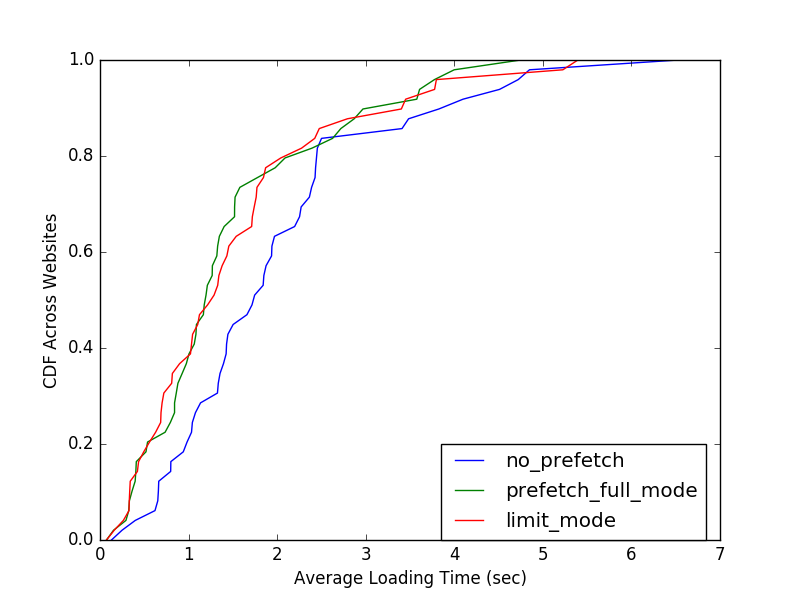
\includegraphics[width=0.48\textwidth]{average.png}  
%	}
%	\subfigure[CDFs of median loading times] {  
%		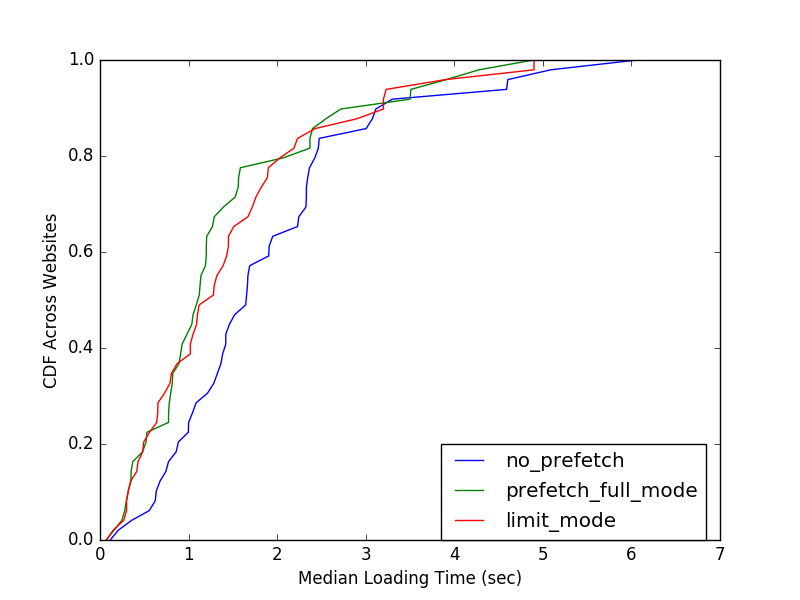
\includegraphics[width=0.48\textwidth]{median.png}  
%	}
%	\caption{CDFs of average loading times and median loading times of 50 websites in full mode, limit mode, and non-prefetching mode.}
%	\label{fig:average}
%\end{figure} 

\begin{figure}[htbp] 
	\centering
	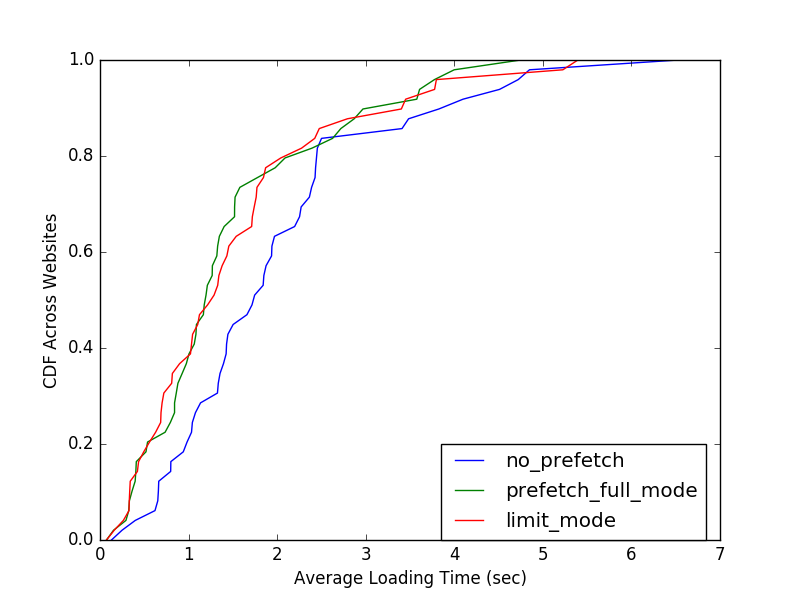
\includegraphics[width=0.5\textwidth]{average.png}  
	\caption{CDFs of average loading times of 50 websites in full mode, limit mode, and non-prefetching mode.}
	\label{fig:average}
\end{figure} 

\begin{figure}[htbp] 
	\centering
	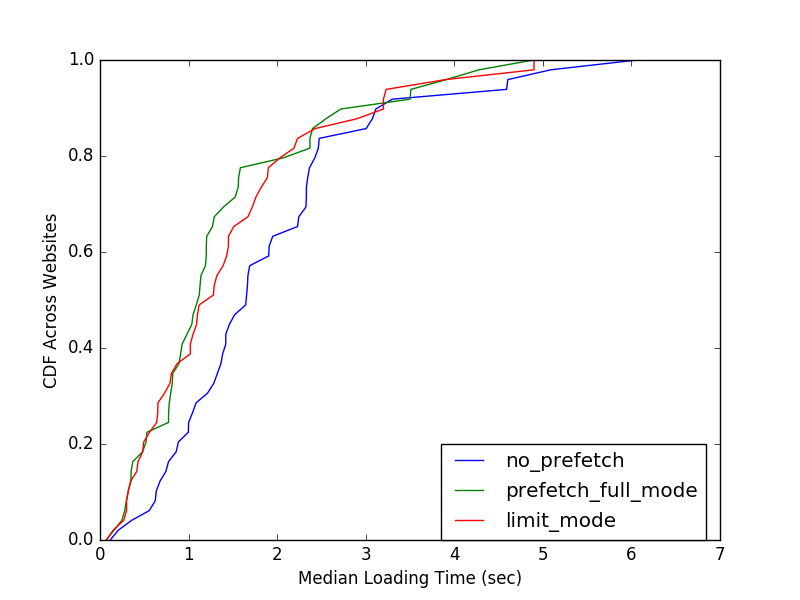
\includegraphics[width=0.5\textwidth]{median.png}  
	\caption{CDFs of median loading times of 50 websites in full mode, limit mode, and non-prefetching mode.}
	\label{fig:median}
\end{figure} 


\subsection{Number of HTTP Reqeusts Prefetched}


We use the same 50 websites from the last experiment to test the number of HTTP requests prefetched in the full mode and the limit mode. For each website, we record the numbers of web requests that are prefetched in both modes. The resulting CDFs are plotted in Fig.~\ref{fig:number_requests}. We can see that the number of requests prefetched in the full mode significantly exceeds the number of requests in the limit mode. In the limit mode, the maximum number of web requests is less than 125, while in the full mode, the maximum number can be as large as 225. For about 80\% of websites, the number of web requests prefetched in the limit mode is less than 50; in the full mode, this fraction is only 40\%.

Our finding implies that the cost of mispredictions in the full mode can be much higher than the cost in the limit mode. While the loading times in the limit mode shown in Fig.~\ref{fig:average} and Fig.~\ref{fig:median} are not significantly less than the times in the full mode, the difference in misprediction costs can be vital. Hence, when the network bandwidth is limited, we suggest using the limit mode instead of the full mode.


\begin{figure}[htbp] 
	\centering
	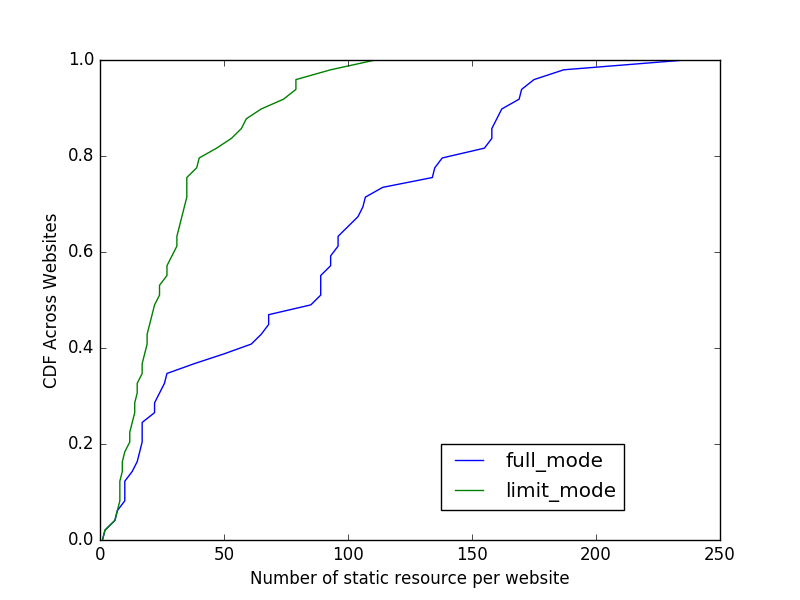
\includegraphics[width=0.5\textwidth]{static_resource.png}  
	\caption{CDFs of the numers of prefetched resources of 50 websites in full mode and limit mode.}
	\label{fig:number_requests}
\end{figure} 











